\subsection{Autres réalisations}
Au cours du projet, plusieurs outils alternatifs ont été explorés. Bien que ces développements n'aient pas été intégrés à la solution finale, ils ont contribué à l'avancement du projet et à la prise de décision. Cette section détaille ces réalisations.

\subsubsection{Drones Crazyflie}
Initialement, les drones Crazyflie 2.1 de Bitcraze ont été envisagés pour les tests en vol. Ces drones sont compacts, abordables et bénéficient d'une communauté active. Une simulation sous Gazebo a été mise en place pour tester virtuellement les algorithmes. Un simulateur existant pour un drone a été téléchargé et modifié pour prendre en charge deux drones. Cependant, cette configuration présentait des limitations : les deux drones étaient pilotés par la même commande et le contrôle s'effectuait en vitesse, sans qu'un pilotage par roulis, tangage et lacet (roll, pitch, yaw) n'ait pu être atteint. Finalement, cette piste a été abandonnée suite à la réorientation du projet vers les robots terrestres. Les travaux sur les drones Crazyflie sont néanmoins présentés en annexe \ref{annexe:tuto_crazyflie}.
Les deux Crazyflie simulés dans Gazebo sont visibles sur la figure \ref{fig:crazyflie_gazebo}.

\begin{figure}[H]
    \centering
    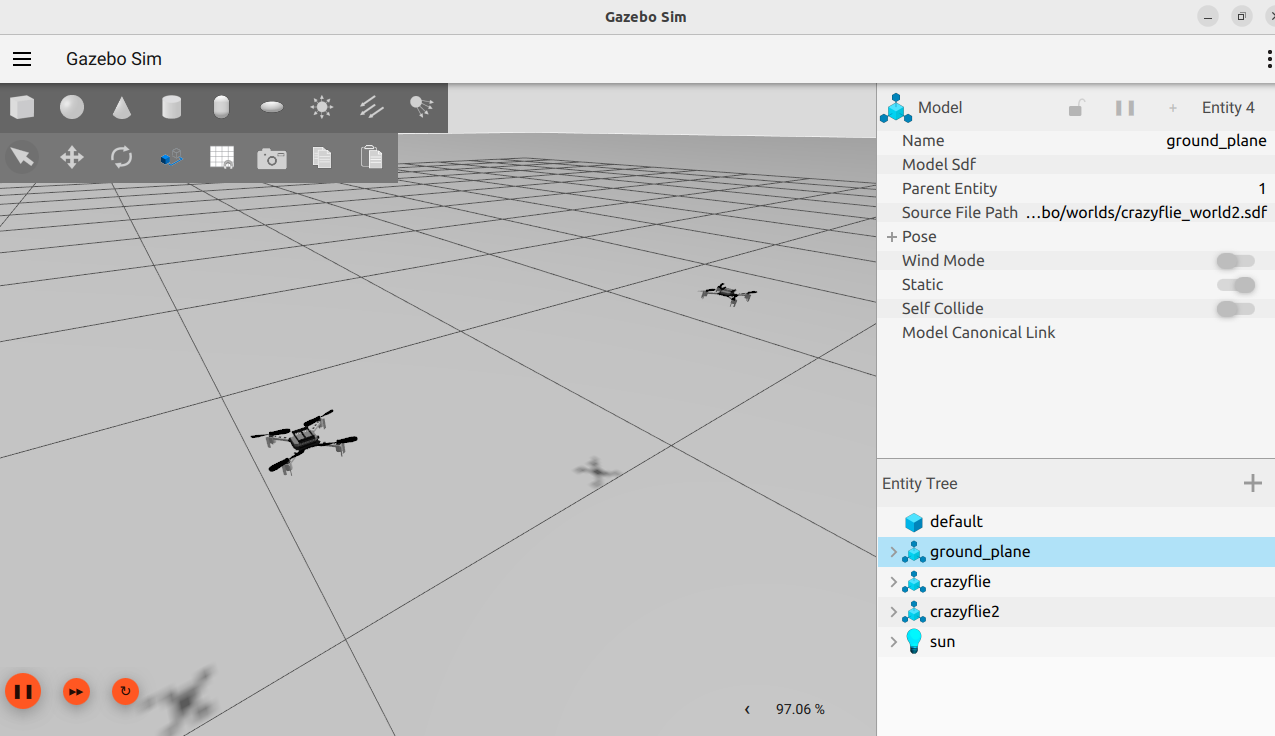
\includegraphics[width=0.8\textwidth]{10-Descriptions_réalisations/Outils/pic/simu_eswarm.png}
    \caption{Simulation de deux drones Crazyflie dans Gazebo.}
    \label{fig:crazyflie_gazebo}
\end{figure}

\subsubsection{Turtlesim}

Les premières versions des algorithmes de contrôle d'essaim ont été testées avec le simulateur Turtlesim de ROS2. Il s'agit d'un outil simple simulant des robots mobiles dans un environnement 2D. Chaque robot, représenté par une tortue, peut se déplacer et tourner sans contrainte, comme des robots à roues Mecanum. Pour se rapprocher des conditions réelles, des nœuds ROS ont été développés pour récupérer les positions des tortues et les republier avec les paramètres de \gls{qos} adéquats. Les tortues ont été renommées pour correspondre aux noms des robots réels, et les topics ont été harmonisés, facilitant ainsi la transposition du code vers le cas réel. Le simulateur Turtlesim est illustré par la figure \ref{fig:turtlesim}.
\begin{figure}[H]
    \centering
    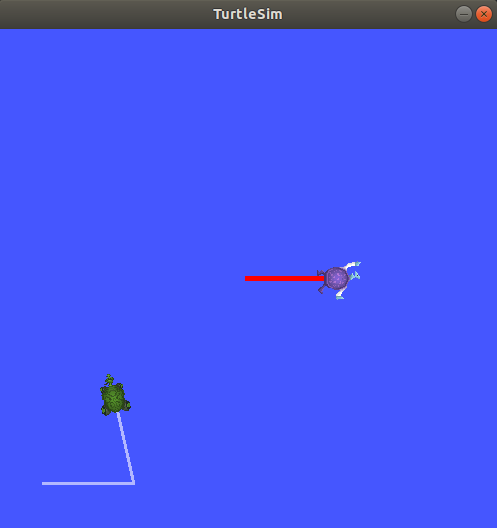
\includegraphics[width=0.4\textwidth]{10-Descriptions_réalisations/Outils/pic/turtlesim.png}
    \caption{Simulation de robots dans Turtlesim.}
    \label{fig:turtlesim}
\end{figure}